\section{Results}
\subsection{Dataset Description}
The data for our case study was collected from the California Report Card between January 18th to April 20th.
We also conducted an independent reference survey using SurveyMonkey's paid random panel system between March 8th and March 14th.
As mentioned, ratings of six political issues were collected on a 13-point letter grade scale (A+,A,...,F) and for analysis we 
mapped these ratings linearly onto a scale from 0 to 1, with an F as 0 and A+ as 1.  Participants also had
the option to ``skip'' issues (not assign a grade).
There were 1575 participants from the CRC and 611  participants from SurveyMonkey.  Rating activity is summarized below.

{\centering\scriptsize
\begin{tabular}[!ht]{ l | r | r | r | l }
Issue & No Change & Change & Skip & Median\\
\hline
\hline
  \multicolumn{5}{l}{\textbf{CRC}}\\
  \hline
  Obamacare & 749 & 223 & 593 & B (0.6667) \\
  \hline
  K12 & 849 & 172 & 544 & C+ (0.5000) \\
  \hline
  College & 923 & 139 & 503 & C- (0.3333)\\
  \hline
  Immigration & 693 & 105 & 767 & C (0.4167)\\
  \hline
  Marijuana & 881 & 118 & 566 & C (0.4167) \\
  \hline
  Marriage Rights & 929 & 105 & 531 & B+ (0.7500)\\
\hline
\hline
\multicolumn{5}{l}{\textbf{Reference}}\\
\hline
  Obamacare & 498 & - & 113 & B (0.6667) \\
  \hline
  K12 & 561 & - & 50 & C (0.4167)\\
  \hline
  College & 573 & - & 38 & C- (0.3333)\\
  \hline
  Immigration & 375 & - & 236 & C+ (0.5000) \\
  \hline
  Marijuana & 498 & - & 113 & C (0.4167) \\
  \hline
  Marriage Rights & 554 & - & 57 & B+ (0.7500)
\end{tabular}\\[1\baselineskip]
}

For any given political issue, between 10\% and 20\% of those who assigned ratings registered a rating change.
In all, 556 out of the 1575 CRC participants changed their rating at least once (Figure \ref{change-1}).
We also found that the aggregate results of the reference survey matched the CRC nearly perfectly.
On only two of the question (K12 and Immigration), we found a observed differences which were both less than a letter grade (+ or -).

\begin{figure}[h]
\hspace*{-2em}
    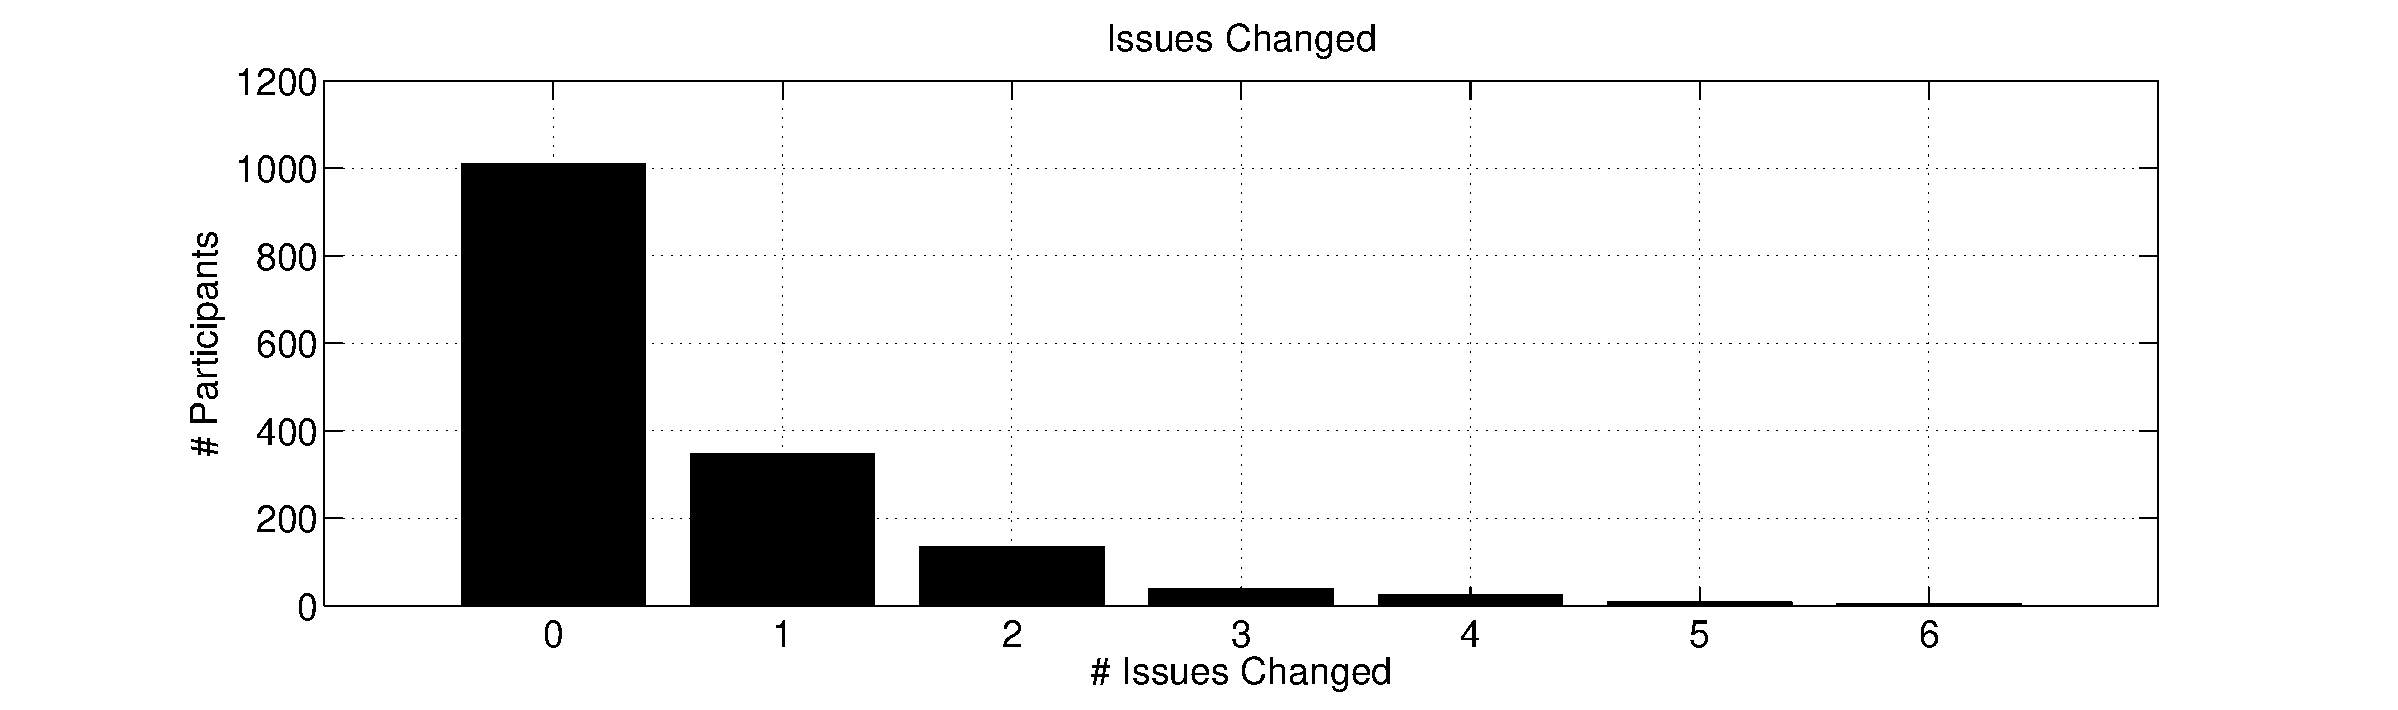
\includegraphics[scale=.25]{../plots/change-1.eps}
    \hspace*{-2em}
    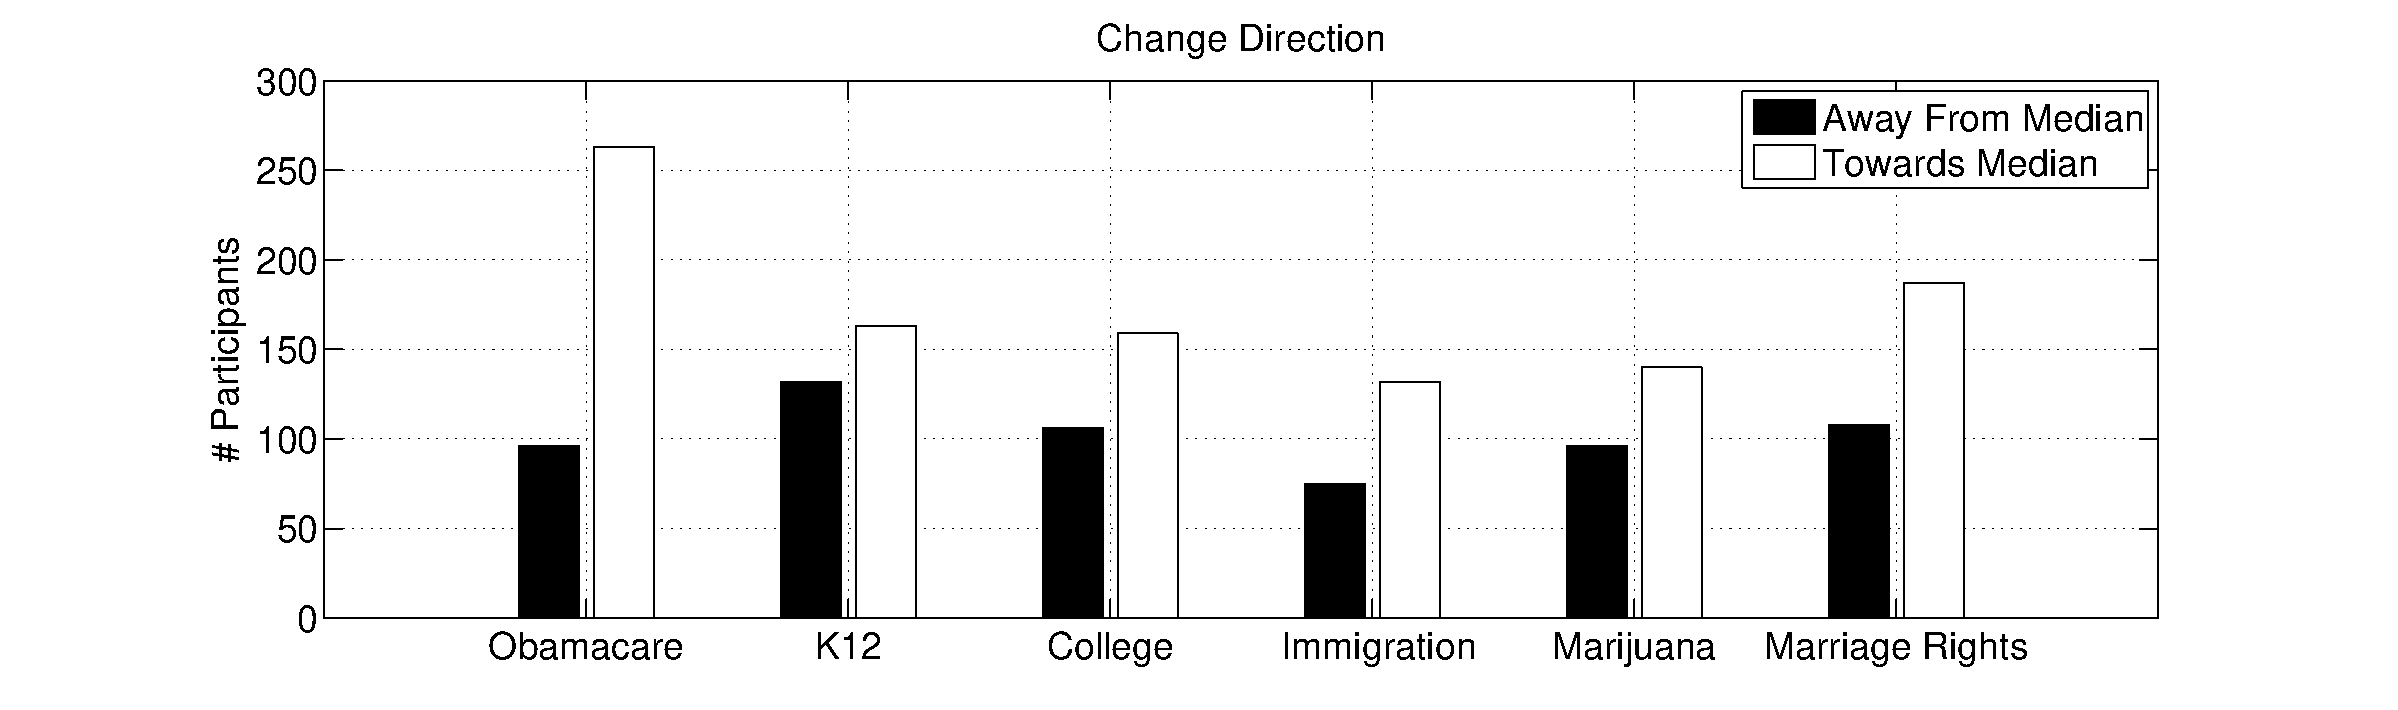
\includegraphics[scale=.25]{../plots/change-2.eps}
      \caption{Among CRC participants, 65\% changed none of their ratings, 22.0\% changed one rating, 8.6\% changed two, and 6.5\% changed three or more. The lower figure omits those who didn't change and indicates that majority of rating changes were towards the median.}
      \label{change-1}
      \vspace{2em}
\end{figure}

\subsection{Analysis}

\subsubsection{Correlation vs. Absolute Deviation}
\label{exp-robust}
In Section \ref{ht}, we argued that using correlation as a test statistic can lead to erroneous conclusions of social influence bias, and proposed testing the absolute deviations around the median.
We ran an experiment to illustrate the problems of using correlation instead of absolute deviation.
In this experiment, we iterated through the initial ratings each of participants in the change group $P_c$.
For each rating, we randomly sampled a final rating from group $P_n$, the ones that did not change.
In this model, since we sample final ratings from the no change group, we know that the social influence bias hypothesis is not true, since in distribution those who changed their ratings and those who didn't are exactly the same.
However, when we calculate the pearson correlation coefficient between $g_f[j] - m[j]$ (the set of differences between the final grade and the median) and $g_i[j] - m[j]$ (the set of differences between the initial grade and the median), we find statistically significant correlations.

{\centering
\scriptsize
\begin{tabular}[!ht] { r | r | r }
\label{ref-2}
  Issue & corr & p-val \\
  \hline
  \hline
  Obamacare &  0.709 & 5.2e-56 \\
  \hline
  K12 & 0.659 & 4.73e-38 \\
  \hline
  College & 0.673 & 2.26e-36 \\
  \hline
  Immigration & 0.704 & 2.95e-32\\
  \hline
  Marijuana & 0.689 & 1.42e-34\\
  \hline
  Marriage Rights & 0.679 & 3.27e-41 \\
\end{tabular}\\[1\baselineskip]
}
There is a natural tendency for ratings to group around the median and the correlation coefficient does not account for this.
However, if we measure the absolute deviation, we will find there is no statistically significant difference between the absolute deviations since they are the same in distribution.

\subsubsection{Significance in CRC}
Using the non-parametric test proposed in Section \ref{ht}, we tested the hypothesis of whether rating changes led to significantly more concentration around the median.
In our first experiment (Figure \ref{mdev-1}), we tested the absolute deviations of the CRC participants.
We compared the group of participants that did not change their ratings to the group that changed their ratings.
We found that while there were no statistically significant differences between the initial ratings of the two groups, the final ratings of the group that changed were statistically significantly more concentrated than both their own initial ratings and the ratings of the no change group.
On average, the ratings were $19.3\%$ closer to the median in the change group.
The results of the hypothesis test for the set of participants who changed their ratings $P_c$ and those who did not $P_n$ are (we denote initial grades from $P_c$ as $i$ and final as $f$):
\begin{figure}[h]
\centering
    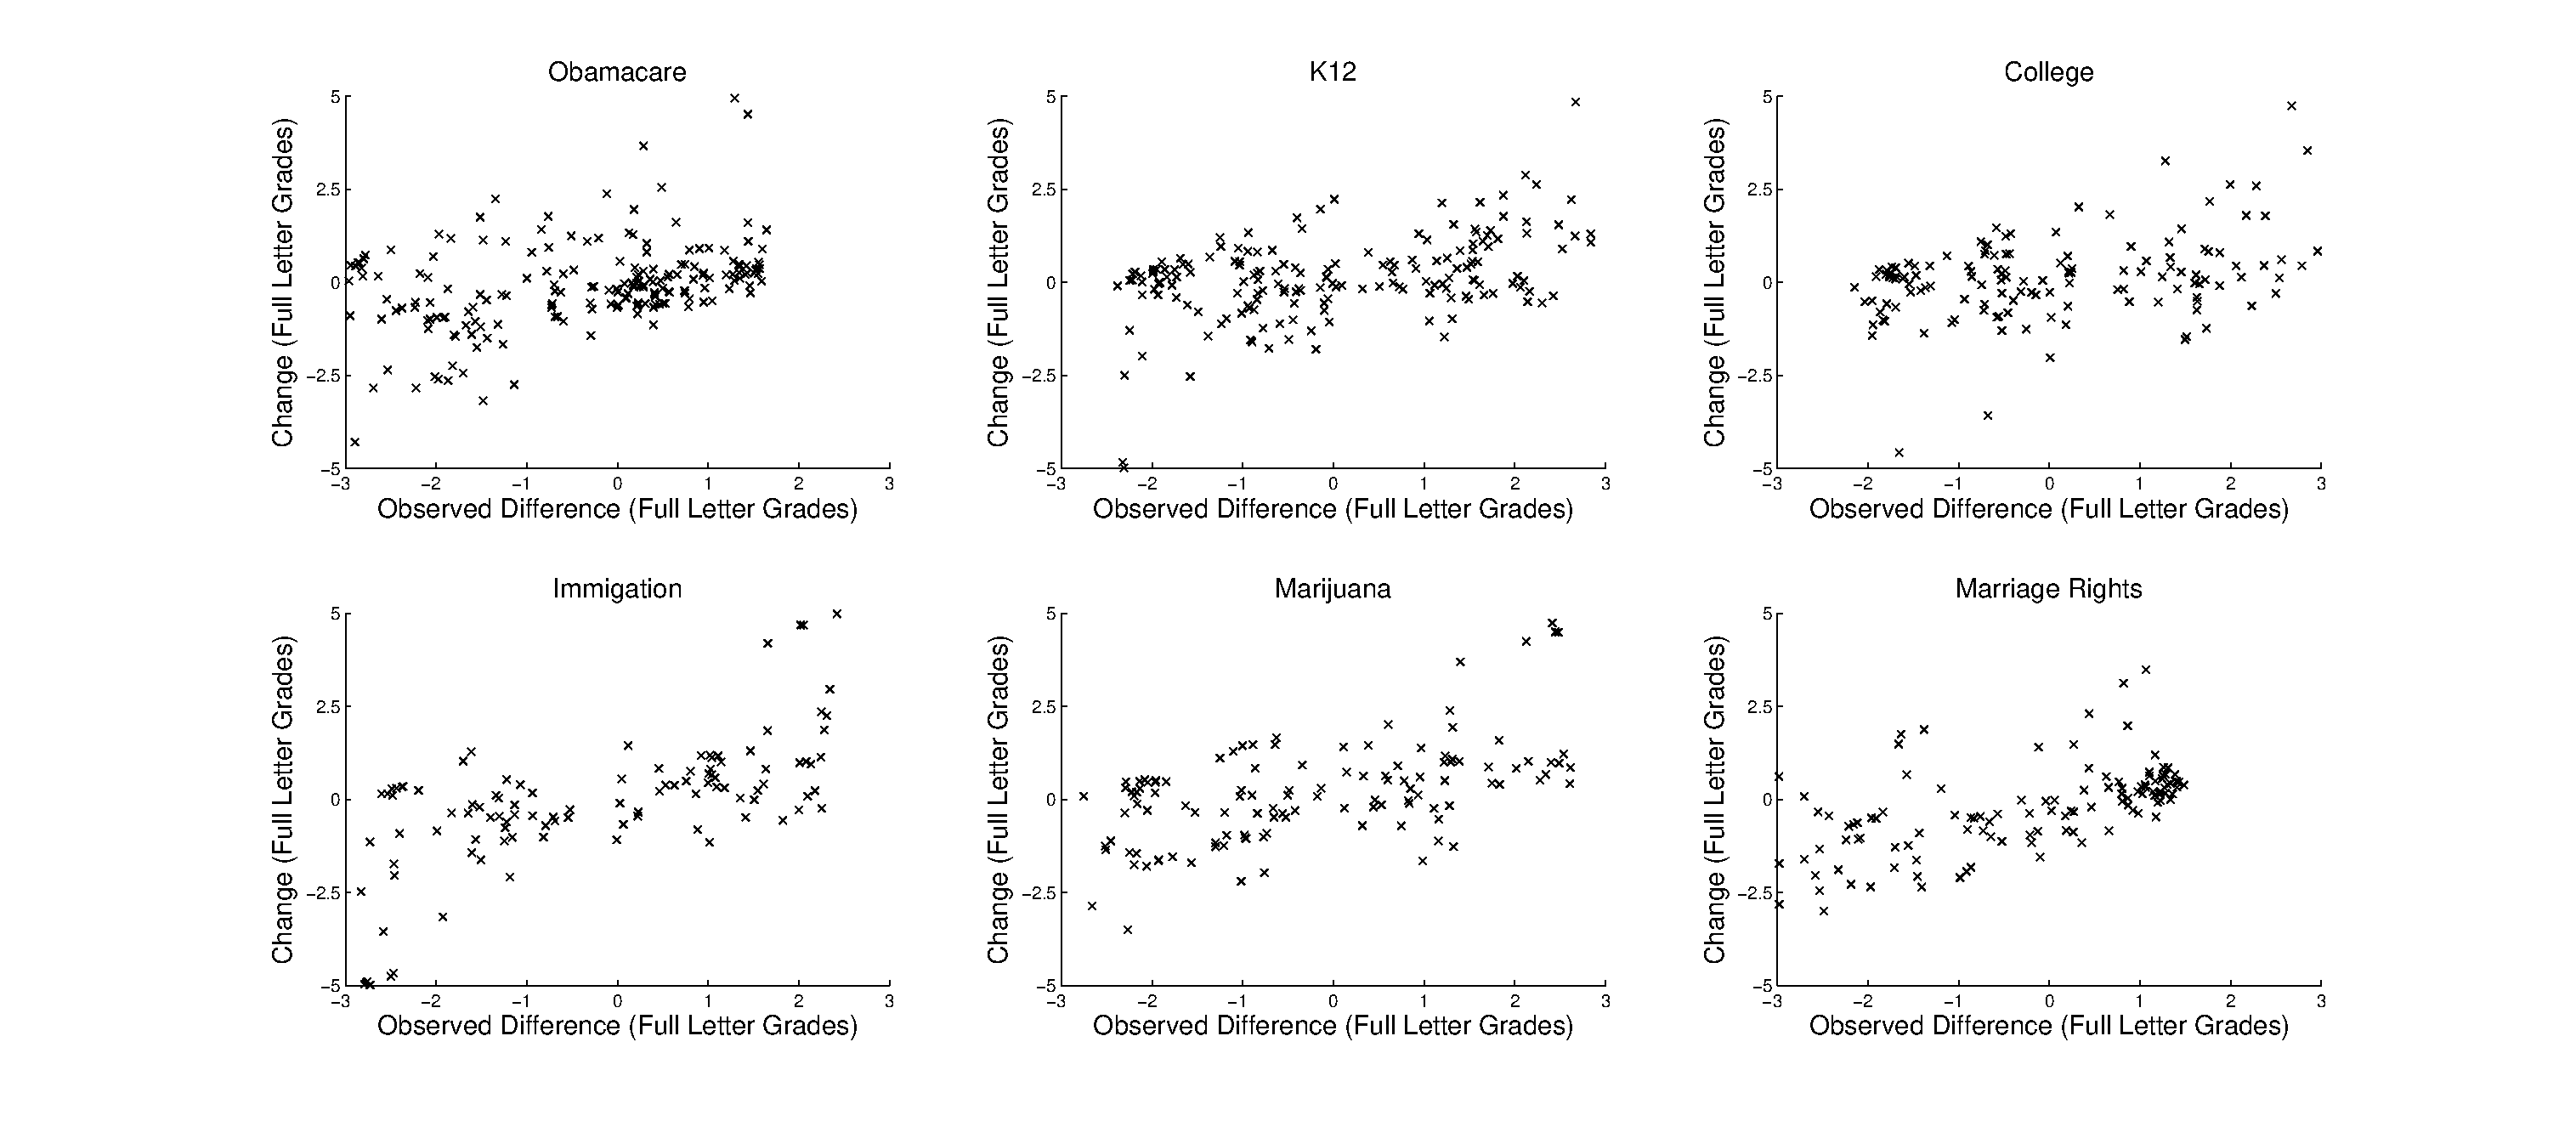
\includegraphics[scale=0.25]{../plots/bias-1.eps}
      \caption{For those participants that changed their ratings, final ratings were significantly more concentrated around the median than their initial ratings. In addition, these ratings are more concentrated than the ratings for those who didn't change.}
      \label{mdev-1}
\end{figure}

{\centering
\scriptsize
\begin{tabular}[!ht] { r | r | r }
\label{dev-2}
  Issue & p-val($P_c$ vs. $P_n$) & p-val($i$ vs. $f$) \\
  \hline
  \hline
  Obamacare &  0.0286 & 0.0161 \\
  \hline
  K12 & 2.1314e-06 &  0.0086 \\
  \hline
  College & 1.3033e-04 & 0.0415 \\
  \hline
  Immigration & 7.3456e-07 &4.4170e-05\\
  \hline
  Marijuana & 2.7549e-10 & 4.2560e-05\\
  \hline
  Marriage Rights & 3.5946e-06 & 2.4644e-10 \\
\end{tabular}\\[1\baselineskip]
}

These results are consistent with social influence bias.
When participants change their ratings, they are more likely to concentrate around the median.
It is however an encouraging and positive result that the two groups of participants $P_n$ and $P_c$ are very similar in terms of initial ratings, and the data suggests that a participant's susceptibility to social influence is not correlated with initial ratings.

\subsubsection{Comparison to Reference Survey}
In our second experiment (Figure \ref{mdev-2}), we apply the same testing procedure to compare the ratings from the CRC to to those in the reference survey.
We compare absolute deviations of the group of participants who changed their ratings in the CRC against participants from the reference survey.
The final ratings were 12.0\% closer to the median in the CRC change group than in the reference survey.
We also found that there was no statistically significant difference between the reference survey and initial ratings.
The results of the hypothesis test for the set of participants who changed their ratings $P_c$ and the reference group $R$ are (we denote initial grades from $P_c$ as $i$ and final as $f$):
\begin{figure}[h]
\centering
    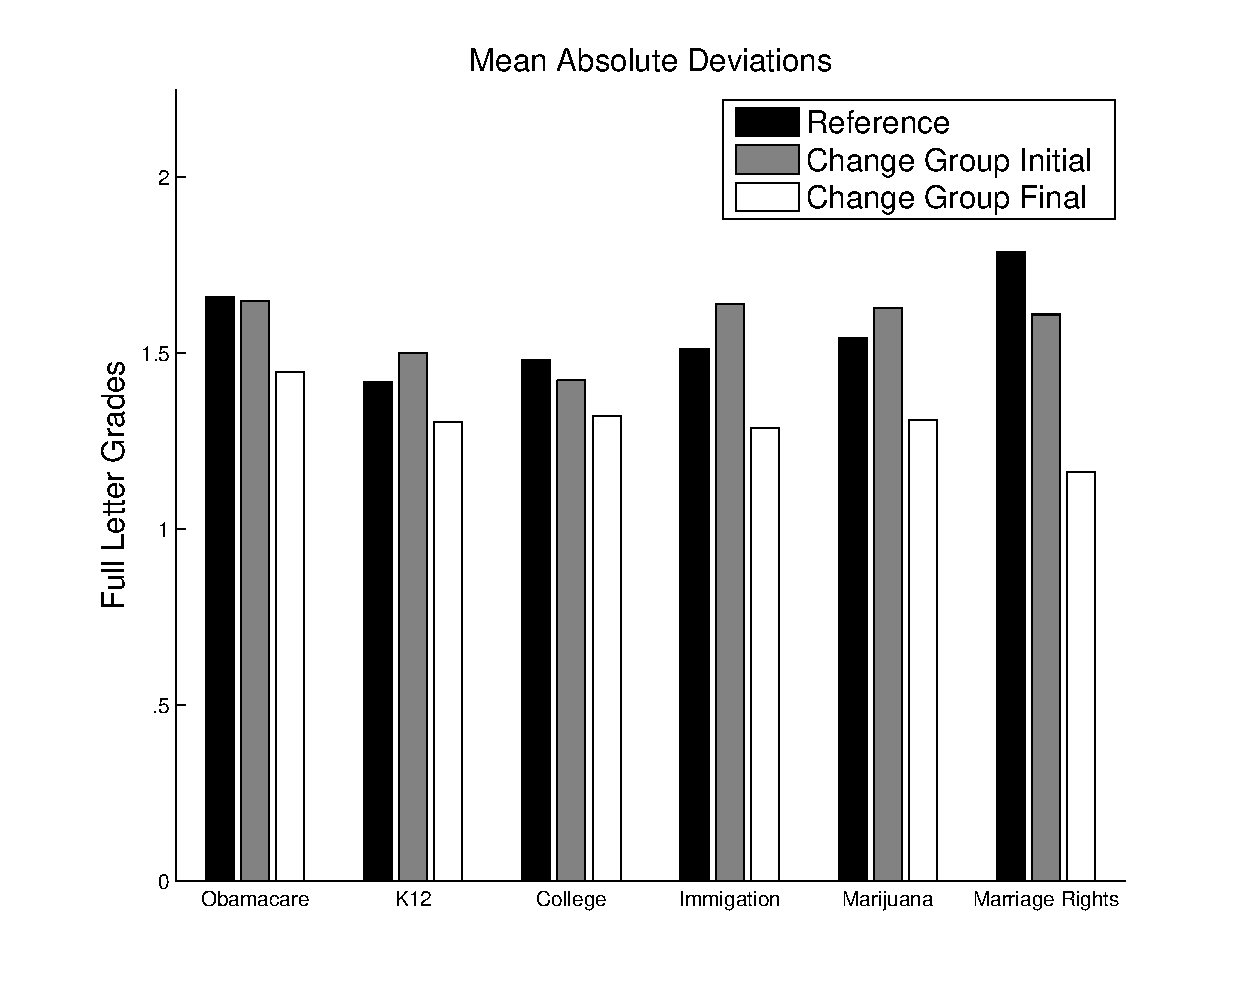
\includegraphics[scale=0.25]{../plots/bias-2.eps}
      \caption{We found that final ratings were significantly more concentrated in the CRC compared to ratings in the reference survey. Similar to Figure \ref{mdev-1}, we found that there was no statistically significant difference between the reference survey and the initial ratings.}
      \label{mdev-2}
\end{figure}

{\centering
\scriptsize
\begin{tabular}[!ht] { r | r | r }
\label{ref-1}
  Issue & p-val($R$ vs. $i$) & p-val($R$ vs. $f$) \\
  \hline
  \hline
  Obamacare &  0.5386 & 0.0015 \\
  \hline
  K12 & 0.8283 & 0.0097 \\
  \hline
  College & 0.1452 & 0.0091 \\
  \hline
  Immigration & 0.3765 & 1.1787e-04\\
  \hline
  Marijuana & 0.7288 & 9.3111e-06\\
  \hline
  Marriage Rights & 0.2478 & 0.0161 \\
\end{tabular}\\[1\baselineskip]
}

The results of our two experiments are consistent with social influence bias.
We not only found that participants' changed ratings were statistically significantly more likely to concentrate around the median, they were also more likely in comparison to the reference survey.

%\subsubsection{Estimating the Distance From the Null Hypothesis}
%\begin{figure}[ht!]
%\centering
%    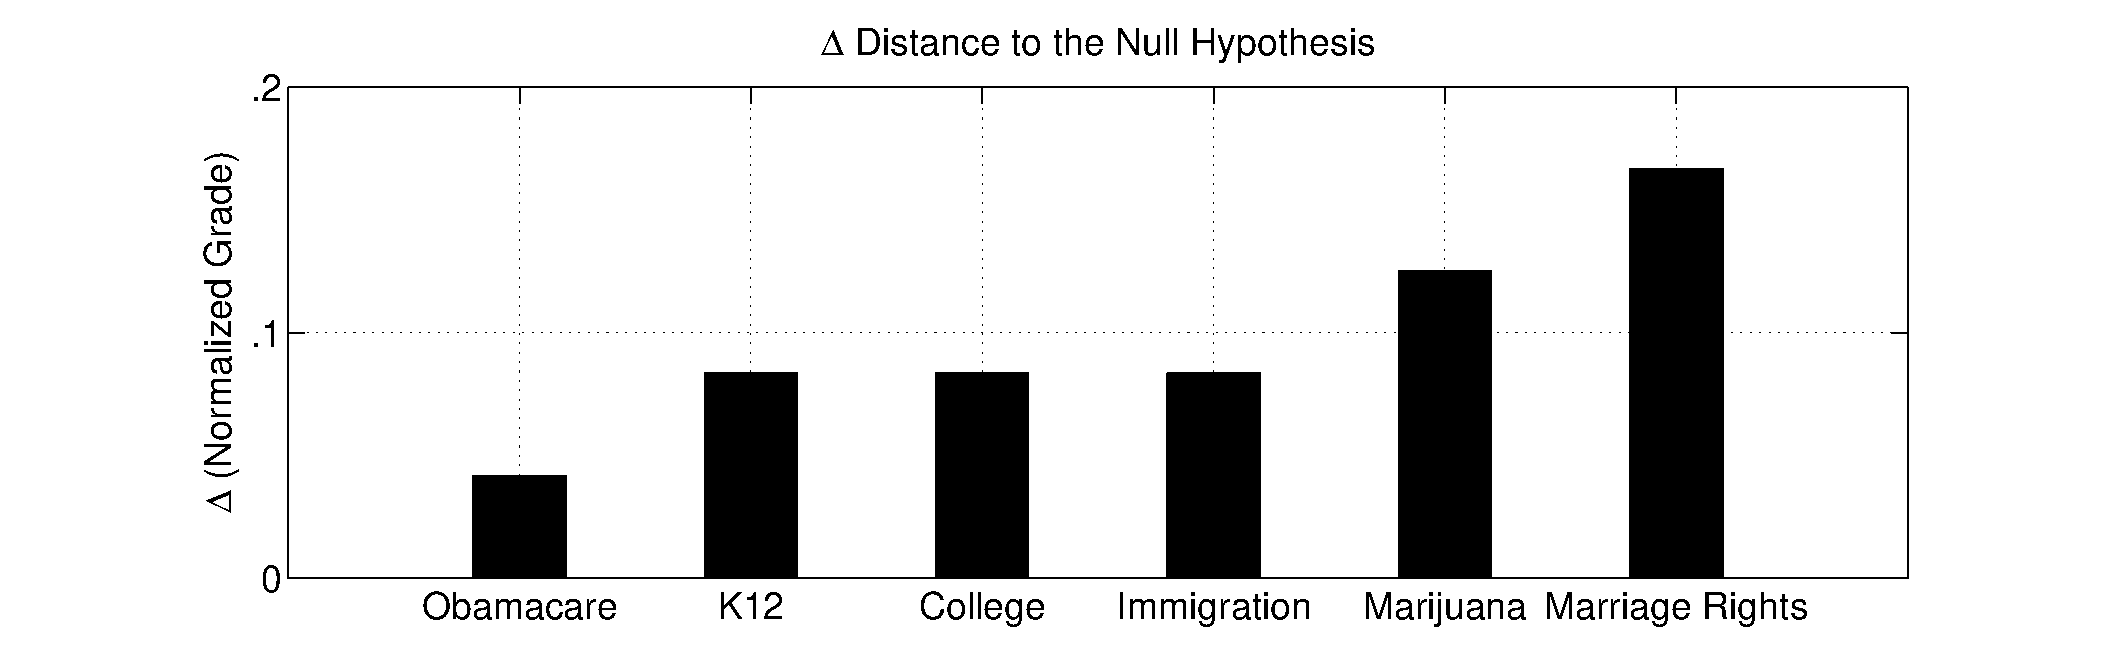
\includegraphics[scale=0.26]{../plots/shift-parameter.eps}
%      \caption{We calculate the shift-parameter $\Delta$ which is the distance from the null hypothesis. Over all issues, we found that ratings the average $\Delta$ was $0.0972$ corresponding to a little more than a +/- grade.}
%      \label{shift-1}
%\end{figure}
%We tested the hypotheses and conclude significant additional concentration of ratings around the median.
%In Section \ref{ht}, we described how we could use the results of the hypothesis test to estimate the $\Delta$ parameter, which quantifies how different the hypothesis is from the null distribution (no social influence bias).
%In other words, how much would we have to spread our ratings around the median to negate the significant biasing result.
%We use $\Delta$ as a measure of social influence bias.

%In Figure \ref{shift-1}, we show the $\Delta$ estimates for each of the issues.
%For the issue about Marriage Rights, we find that parameter is largest at $0.1667$.
%This means that all the final ratings for the Marriage Rights issue would have to be changed by $0.1667$, corresponding to 2/3 of a letter grade eg. difference between B and A-, for us to conclude that there is no social influence bias in the dataset.
%For the other issues, the parameter was smaller indicating less of an effect of social influence bias.
%On average over all issues, the ratings were $0.0972$ to a little more than a +/- grade.

\begin{figure*}[ht!]
\hspace{-7em}
    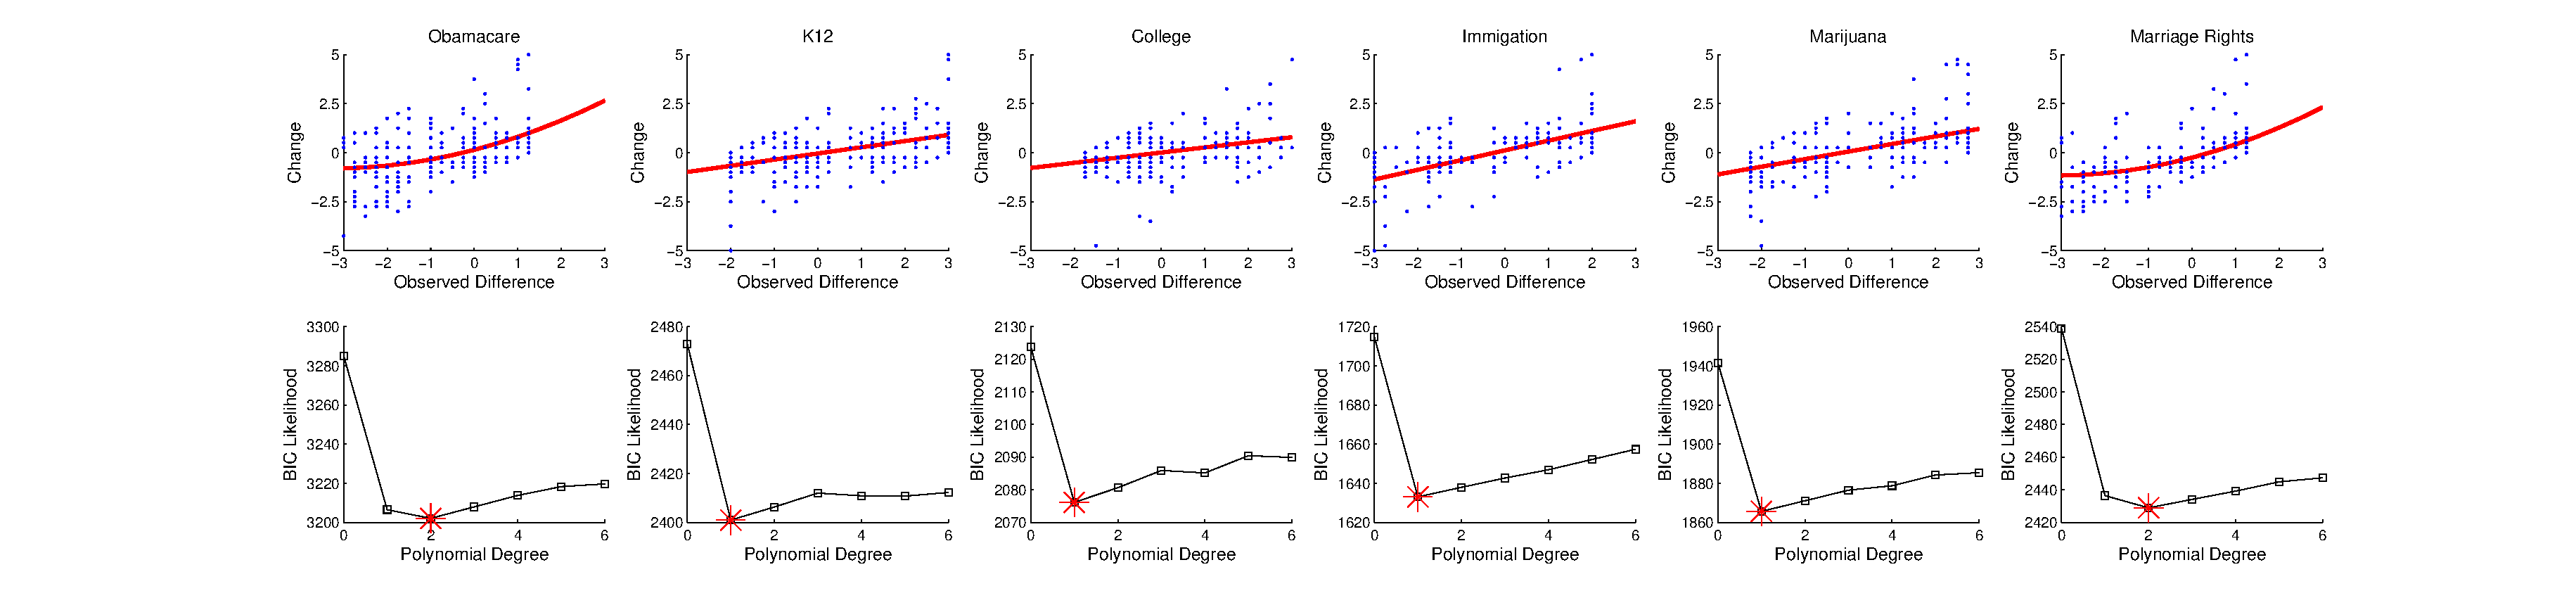
\includegraphics[scale=0.38]{../plots/BIC-optimization.eps}
      \caption{We plot the difference between ratings and the median (X-axis), and the change in rating (Y-axis). We overlay the optimal polynomial model to represent the relationship $f(x) = y$. Below each plot, is the BIC objective function showing how we picked an optimal degree of polynomial.}
      \label{opt-1}
\end{figure*}

\subsection{Mitigation}

\subsubsection{Classifying Final Grades As Changed}
In Section \ref{changemod}, we discussed how we could use logistic regression to estimate the probability that a rating has been changed.
We applied logistic regression, as described in that section, and inferred which ratings were changed.
In Figure \ref{change-pred-1}, as is typically used to evaluate binary classifiers, we show the ROC plot of the logistic regression predictor.
\begin{figure}[h]
\centering
    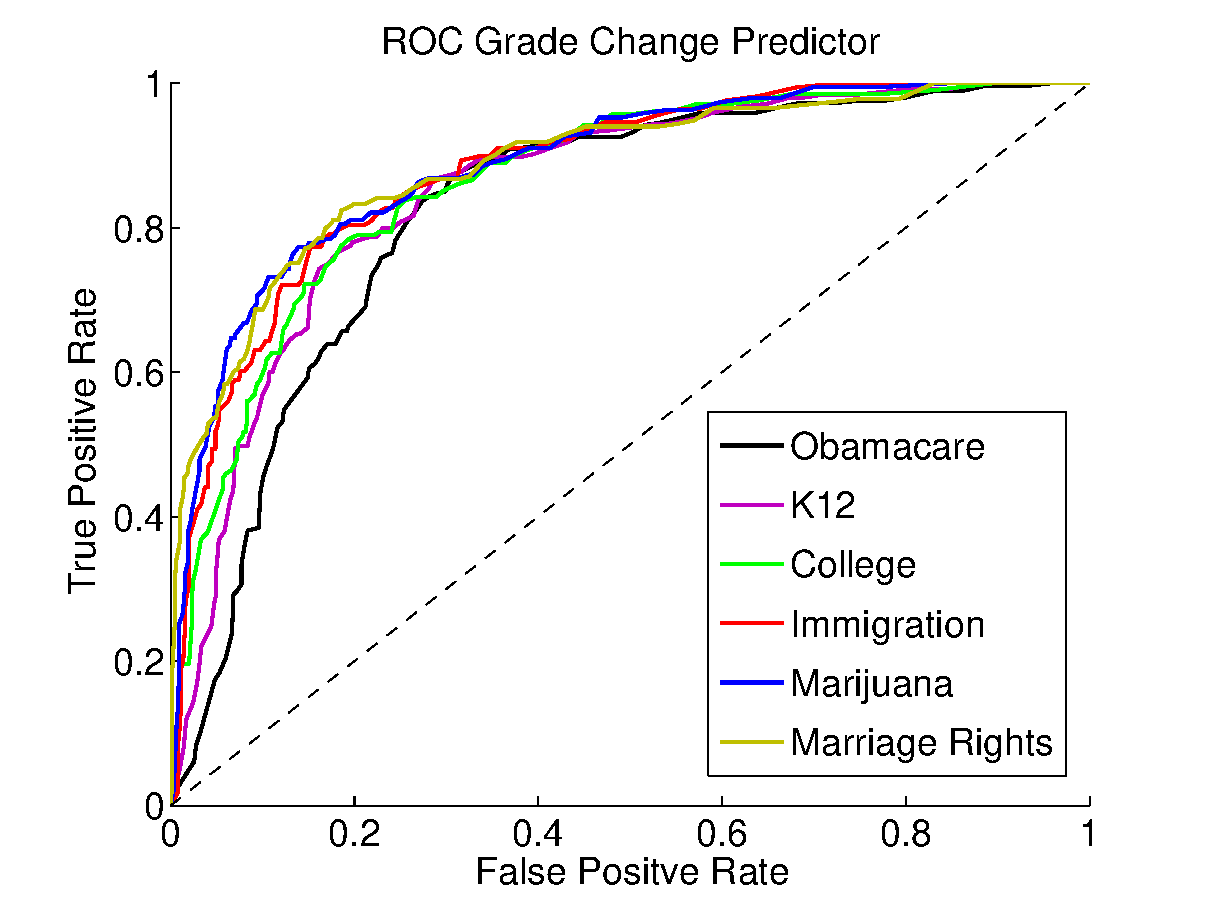
\includegraphics[scale=0.26]{../plots/roc-predicting-changes.eps}
      \caption{This plot shows the true positive rate (correct classifications) as a function of the false positive rate. We find that our prediction is quite accurate, substantially better than random (dashed line) with an average AUC score of 0.8670.}
      \label{change-pred-1}
\end{figure}
The prediction results were quite accurate with average AUC score over all issues of 0.8670.
At the .50 probability threshold (classified as changed if the estimated probability is greater than 0.5), we achieved an average precision of 84.7\% and a recall of 70.0\%.

\subsubsection{Correction Model}
In the first experiment, we train the polynomial/BIC correction model proposed in Section \ref{changemod}, and evaluated it in terms of RMSE (Figure \ref{poly-1}).
We look at model only for those changed their grades, and measure how accurate is the model in predicting the grade changes.
We held out a random 20\% of rating triplets and calculated the inference error in the correction model.
We found that on average over all issues the RMSE was $0.1286$ which corresponds to a little bit more than a + or - grade.

In the second experiment, we simulated a true post-learning setting.
We used the logistic regression model to predict the probablity that the participant changed their grade.
Then, if this probability was above a threshold, we used 70\% which was determined empirically, we then apply the polynomial correction model
to infer the unbiased grade.
Since the majority of participants did not change their grades, it would not be correct to simply measure RMSE error which would average predictions for those who changed and did not change.
Thus, we invert the significance test proposed in Section \ref{ht}, to calculate a parameter $\Delta$ which measures the distance from the null hypothesis.
That is, how much would we have to shift the distribution of absolute deviations so the null hypothesis (of no social influence bias) is the most likely hypothesis.
In Figure \ref{poly-1}, we show a before and after for apply the correction model.
We found that there was on average a 76.3\% reduction in $\Delta$ for the entire pipeline predicting a change and then correcting for it. 

\begin{figure}[h]
\hspace*{-2em}
    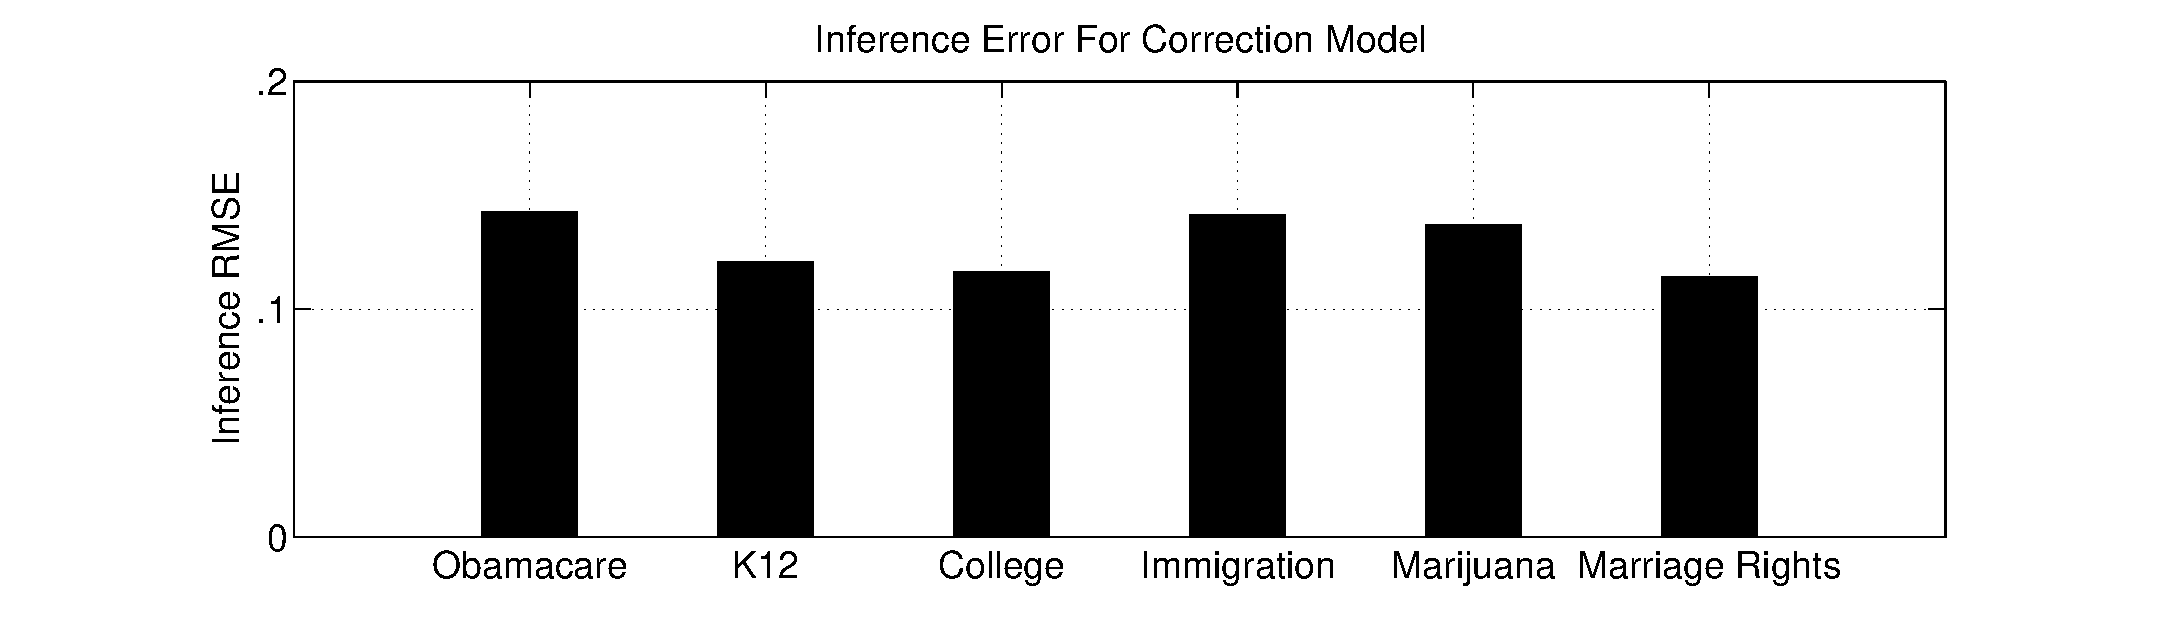
\includegraphics[scale=0.27]{../plots/prediction-error.eps}
    \hspace*{-2em}
    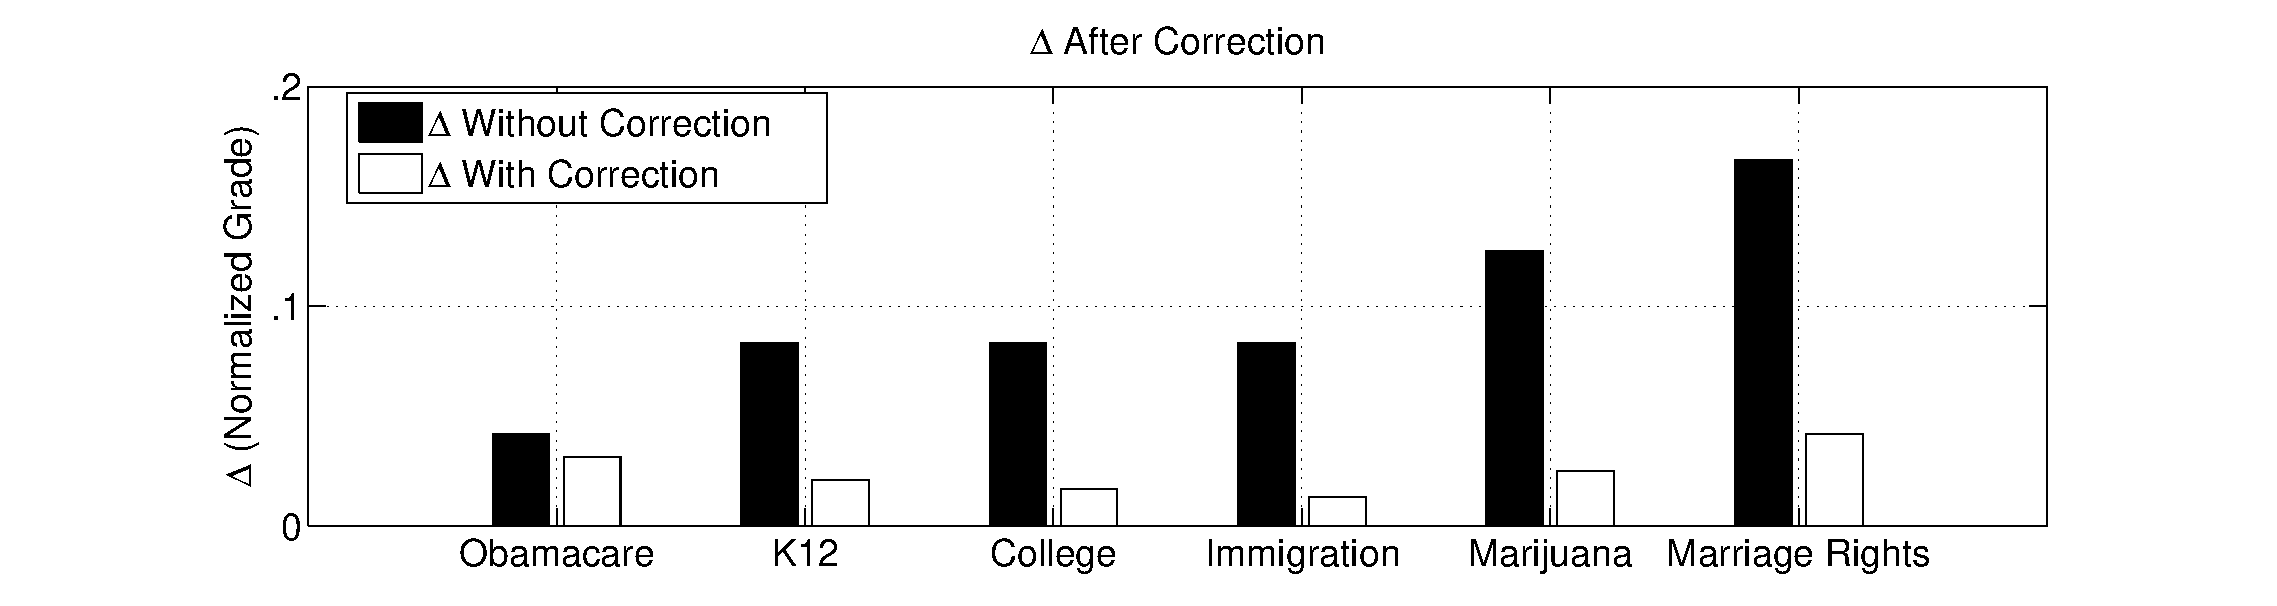
\includegraphics[scale=0.26]{../plots/shit-2.eps}
      \caption{We measured the RMSE prediction error of the polynomial model. We found that we could predict changes in all of the issues with less than 2/3 of a letter grade RMSE error. In the lower figure, we applied this model to correct for the social influence bias and found that, on average, we could reduce the effects by 76.3\%}
      \label{poly-1}
\end{figure}

\subsubsection{Prediction Model}
We applied the prediction from Section \ref{changemod} and the results are shown in Figure \ref{opt-1}.
Our model search and optimization through the BIC discovered that for four out of the six issues, K12, College, Immigration, and Marijuana, the model was linear.
This suggests homogeneity in positive and negative social influence effects for these issues.
What this implies is that on average participants who rated above the median and below the median moved towards the median with the same magnitude.
However, for Obamacare and Marriage Rights, we found that the relationship was quadratic.
Interestingly enough, over the domain of changes, the learned quadratic function had steeper slope for ratings above the median.
In other words, participants who initially rated the state higher than the median had a more significant tendency to change downwards, in comparison to the upward tendency of those who rated less than the median.

%\subsection{How Many Training Examples?}
%It is important to note that our training set sizes were relatively small. 
%Even with this small size, we were able to find an accurate correction model.
%The caveat is that only a fraction of participants will actually change their ratings during the learning phase.
%In Figure \ref{poly-2}, we plot the optimality of the test error as a function of training set size for the correction model. 
%We define the optimality percentage to be the ratio of the current test error to the best possible test error (test error using all 80\% of the training set).
%We averaged the results over 1000 trials randomly picking a different 80\% for training and 20\% test.
%We found that a surprisingly few training examples could get a reasonably accurate model.
%For the linear models, we found that we could achieve greater than 95\% optimality with only 25 examples.
%For the quadratic models, we required a little bit more data for the same optimality.

%\begin{figure}[h]
%\centering
%    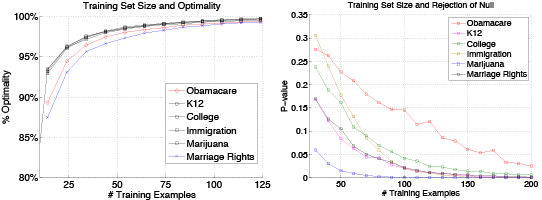
\includegraphics[scale=0.45]{../plots/training-combined.png}
%      \caption{We find that we can train our correction model on less than 50 examples and get a model that on average performs only 5\% worse than a model trained on the full training set. In the second plot, we plot p-values of our significance test as a function of training set size. We find for 5 out of 6 issues we could reject the null with less than 100 examples.}
%      \label{poly-2}
%\end{figure}

%We can also look at the relationship between training set size and the analysis phase, where we are testing the statistical significance of the spread of the ratings around the median.
%Specifically, we can measure the average number of training examples needed before we can reject the null hypothesis at $p<0.05$.
%In this dataset, we find that determining the significance of social influence bias requires more training examples than predicting its effects. 



